
\chapter{Related Work}

This chapter will give a brief introduction to neural networks and time delay neural networks, as well as an introduction automated speech recognition with hidden Markov models. These are the necessary building blocks for the work presented in this thesis. At the end of this chapter, we will also briefly present research that directly inspired this work. 

\section{Neural Networks}

In machine learning research, the goal of a \textit{neural network} is to approximate arbitrary functions. The basic idea of neural networks, so called \textit{perceptrons}, were first introduced by Rosenblatt in \cite{rosenblatt1958perceptron}. While the first neural networks were biologically motivated, neural networks can be interpreted as composition of functions. The relation between these functions forms a directed graph. In this work, we will only cover \textit{feed forward neural networks}. They are called feed forward neural networks because there are no feedback connections: The relation between all functions in the neural network forms an acyclic directed graph. Feed forward networks are an important building block for many machine learning applications. 
\\
More formally, as described in \cite{Goodfellow-et-al-2016}, a feed forward neural network can be described as a model $y = f^*(x, \theta)$, approximating an existing function $y = f(x)$. In this example $x$ is the input, $y$ is the output and $\theta$ are the model parameters which are learned during training. $f$ is the function to approximate and $f^*$ is a composition of many functions with the parameters $\theta$. 
\\
In practice, the functions composing a feed forward neural network are often simply chained, so that their relation graph simply forms a path. In this case, the functional components are called layers. A feed forward neural network of this form with $n$ layers can be written as follows:

\[
y = f^*_n \dots (f^*_2(f^*_1(x, \theta_1), \theta_2) \dots, \theta_n)
\]

For this type of neural network, $f^*_1$ is applied to the input, then $f^*_2$ is applied to the output of $f^*_1$, until the final layer is reached. The output of the final layer is the output of the neural network. Figure \ref{fig:simple_feed_forward_nn} shows a graph based representation of such a neural network. Each node represents a function, arrows represent data flows. 

\begin{minipage}{\linewidth}
	\makebox[\linewidth]{
	\begin{tikzpicture}[x=1.5cm, y=1.5cm, >=stealth]
	
	\node [every neuron] (n0) at (0*1-1,2.5-0) {$x$}; 
	\node [every neuron] (n1) at (1*1-1,2.5-0) {$f^*_1$}; 
	\node [every neuron] (n2) at (2*1-1,2.5-0) {$f^*_2$}; 
	\node [neuron hmissing] (n3) at (3*1-1,2.5-0) {}; 
	\node [every neuron] (n4) at (4*1-1,2.5-0) {$f^*_n$}; 
	\node [every neuron] (n5) at (5*1-1,2.5-0) {$y$}; 
	
	\draw [->] (n0) -- (n1);
	\draw [->] (n1) -- (n2);
	\draw [->] (n2) -- (n3);
	\draw [->] (n3) -- (n4);
	\draw [->] (n4) -- (n5);
	
	\end{tikzpicture}
	}
	\captionof{figure}{Simple graphical interpretation of feed forward neural network}
	\label{fig:simple_feed_forward_nn}
	\hspace{1cm}
\end{minipage}


Even with this simplification, it has been shown that such a feed forward neural network can approximate any function with any desired accuracy. This is called the \textit{universal approximation theorem}, the proof can be found in \cite{hornik1989multilayer}. The caveat is finding the correct function $f^*_n$ to use in each layer and the correct parameters $\theta_n$. Also, finding the function to approximate is non-trivial in the first place. We will discuss these problems in the next sections. 

\subsection{Designing Neural Networks}

In practice, neural network layers are often formed by combining an affine transformation with a non-linear function. Since affine transformations of data vectors can be interpreted as matrix-vector multiplications, we can write a layer function in the following way, where $x_k$ is the input vector for $k$th layer, $W_k$ is the matrix defining the affine transformation of the $k$th layer, and $\varphi$ is a non-linear activation function of layer k.
\[
f^*_k(x_k) = \varphi_k(W_k x_k)  
\]
The count of layers, as well as the size of each $W_k$ are design decisions and depend on the task. We call the count of layers \textit{depth} of a neural network, and count of rows in $W_k$ the \textit{width} of layer $k$. 

\subsubsection{Activation Functions}

Non-linear activation functions, or simply \textit{activation functions}, can be roughly classified into two groups: Activation functions which are applied element-wise and thus do not change the dimension of the data, as well as activation functions which are applied on groups of elements of the input vector and change the dimension. The latter case is commonly fund with so called pooling functions. The choice of the activation function $\varphi$ has significant impact on the performance of a neural network and has been subject to many bodies of research, as summarized in \cite{thoma2017analysis}. In this work, we will only discuss the \textit{ReLU}, \textit{p-norm} and \textit{softmax} activation functions. 

\subsubsection*{Rectified Linear Unit (ReLU)}
% ReLU
\begin{minipage}{0.45\textwidth}
	\[\phi^{ReLU}(x) = \begin{cases}
	0 & x < 0 \\
	x & x \geq 0
	\end{cases}\]
	First introduced in \cite{krizhevsky2012imagenet}, ReLU nonlinearities have proven successful in practice. The computation of ReLU nonlinearity is cheap, also the gradient never saturates for positive values of $x$. For negative values, the gradient is zero, which can be a disadvantage.  
\end{minipage}
\hfill
\begin{minipage}{0.45\textwidth}
\begin{tikzpicture}[baseline=(current bounding box)]
\begin{axis}[xmin=-2,xmax=2,ymin=-2,ymax=2,axis lines = middle,xlabel = $x$,ylabel = $\phi^{ReLu}(x)$,clip = false]
\addplot+[mark=none,blue,domain=-2:0] {0};
\addplot+[mark=none,blue,domain=0:2] {x};
\end{axis}
\end{tikzpicture} 
\captionof{figure}{The ReLU function.}
\end{minipage}
% L2 Pooling

\subsubsection*{P-norm}
\begin{minipage}{0.45\textwidth}
	\[\phi^{Lp}(X) = \sqrt[p]{ \sum_{x \in X}{x^p} } \] 
	The p-norm nonlinearity was described by \cite{zhang2014improving}. This nonlinearity operates on a set $X$ of input elements and reduces them to one. The group size as well as the $p$ are a design parameter. For a fixed $p$ of $2$, the p-norm is also called \text{L2 pooling}.
\end{minipage}
\hfill
\begin{minipage}{0.45\textwidth}
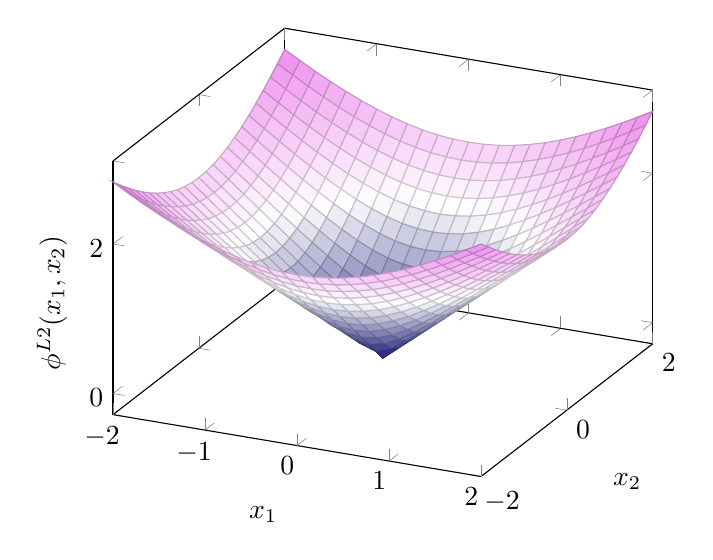
\begin{tikzpicture}[baseline=(current bounding box)]
\begin{axis}[xmin=-2,xmax=2,ymin=-2,ymax=2,xlabel = $x_1$,ylabel = $x_2$,zlabel = $\phi^{L2}({x_1, x_2})$,colormap/violet,clip = false]
\addplot3[surf,samples=25, domain=-2:2]
{sqrt(x * x + y * y)};
\end{axis}
\end{tikzpicture}
\captionof{figure}{Example of p-norm with $p = 2$ and and an input group containing two values}
\end{minipage}

\subsubsection*{Softmax}
\begin{minipage}{0.45\textwidth}
	\[\phi^{softmax}(X)_i = \frac{e^x_i}{ \sum_{x_j \in X} e^x_j } \]
	The softmax activation is defined as an operation over the whole input, but does not reduce the dimension. It maps all output values to a space between $0$ and $1$, preserves the rank of each output and also guarantees that the sum over all outputs is exactly $1$. Therefore it produces a valid probability distribution and is usually used for the last layer of a neural network for classification problems.
\end{minipage}
\hfill
\begin{minipage}{0.45\textwidth}
	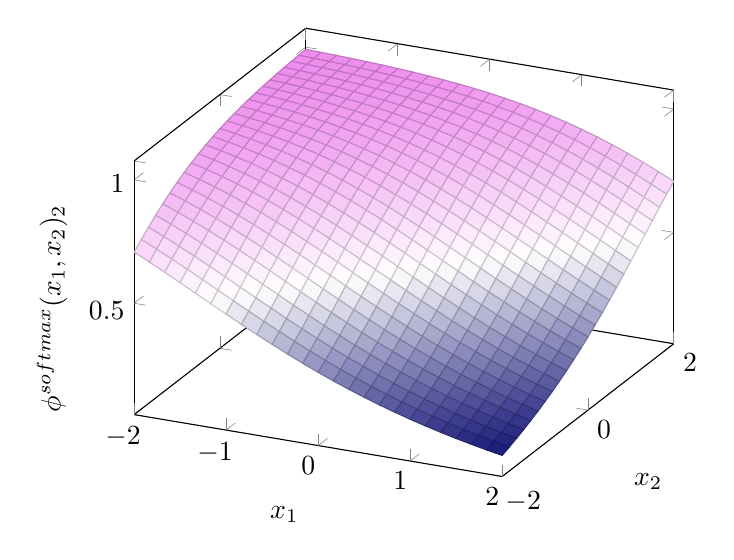
\begin{tikzpicture}[baseline=(current bounding box)]
	\begin{axis}[xmin=-2,xmax=2,ymin=-2,ymax=2,xlabel = $x_1$,ylabel = $x_2$,zlabel = $\phi^{softmax}({x_1, x_2})_2$,colormap/violet,clip = false]
	\addplot3[surf,samples=25, domain=-2:2]
	{sqrt(e^y / (e^x + e^y) )};
	\end{axis}
	\end{tikzpicture}
	\captionof{figure}{Example of softmax for an input vector containing two values}
\end{minipage}

\label{ch:realted_work}
\subsection{ASR with HMM-based systems}
\label{ch:HMM_ASR}

This chapter will be focused on how ASR is done with Janus. It will contain: 
\begin{itemize}
	\item A brief introduction to HMM models
	\item A brief introduction to HMM-based ASR tools:
	\begin{itemize}
		\item description of n-gram language models, dictionaries and context-dependent phone models
		\item description of the purpose of an acoustic model
		\item explanation, about how the this component are combined to form a speech recognizer 
		\item example, showing how the language and phone models, as well as the dictionary are combined to form a HMM
	\end{itemize}
	\item A description of the Word-Error-Rate and Frame-Error-Rate metric. 
	\item An explanation about training HMM-based systems using the expected maximisation algorithm. 
\end{itemize}

\subsection{Time Delay Neural Networks}
\label{ch:TDNN}
The goal of this chaper is to provide a short introduction to neural networks, 
as well as explain the concept of TDNNs. It will contain:
\begin{itemize}
	\item A brief intro to MLPs and SGD
	\item Parameter coupling (convolutional neural networks)
	\item Time delay neural networks
	\item Interpretation of TDNNs as FIR filters
\end{itemize}

\subsection{Acoustic Modelling using Neural Networks}
\label{ch:acoustic_modelling}
The goal of this chapter is to describe the approach of using DNNs for acoustic modelling.
The contents will be: 
\begin{itemize}
	\item definition of the acoustic model training as a deep learning problem
	\item different discriminative training strategies
	\begin{itemize}
		\item Binary Cross Entropy loss on existing labels
		\item Bianry Cross Entropy with re-generating the labels, then trianing again
		\item Minimum Bayes Risk and variants, especially State-Minimum-Bayes-Risk
	\end{itemize}
	\item A brief section about common tricks used when trianing DNN acoustic models, 
	especially Exponential Decay/Newbob.
	\item If there is time left: A brief analysis of the 2nd derivative of the loss function
	during gradient descend.
\end{itemize}

\begin{minipage}{\linewidth}
	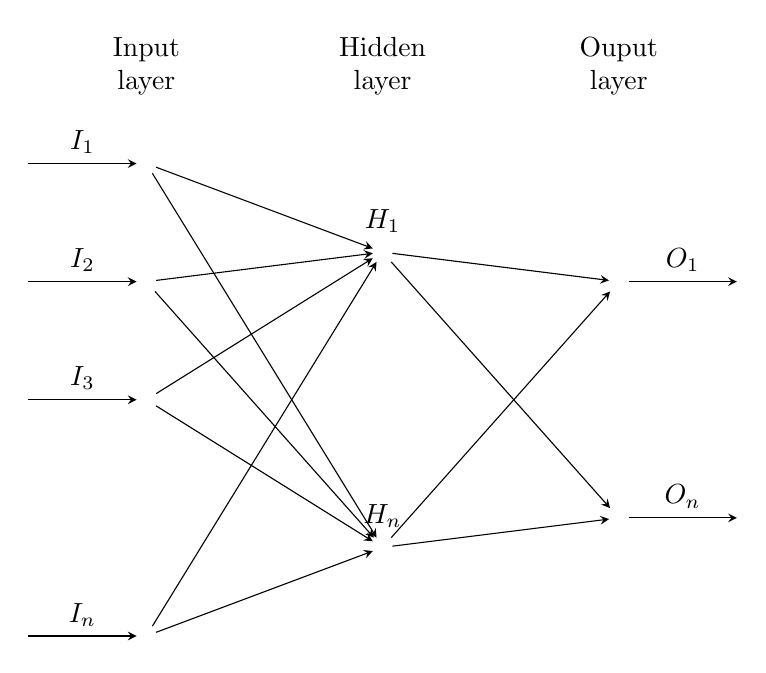
\begin{tikzpicture}[x=1.5cm, y=1.5cm, >=stealth]
	
	\foreach \m/\l [count=\y] in {1,2,3,missing,4}
	\node [every neuron/.try, neuron \m/.try] (input-\m) at (0,2.5-\y) {};
	
	\foreach \m [count=\y] in {1,missing,2}
	\node [every neuron/.try, neuron \m/.try ] (hidden-\m) at (2,2-\y*1.25) {};
	
	\foreach \m [count=\y] in {1,missing,2}
	\node [every neuron/.try, neuron \m/.try ] (output-\m) at (4,1.5-\y) {};
	
	\foreach \l [count=\i] in {1,2,3,n}
	\draw [<-] (input-\i) -- ++(-1,0)
	node [above, midway] {$I_\l$};
	
	\foreach \l [count=\i] in {1,n}
	\node [above] at (hidden-\i.north) {$H_\l$};
	
	\foreach \l [count=\i] in {1,n}
	\draw [->] (output-\i) -- ++(1,0)
	node [above, midway] {$O_\l$};
	
	\foreach \i in {1,...,4}
	\foreach \j in {1,...,2}
	\draw [->] (input-\i) -- (hidden-\j);
	
	\foreach \i in {1,...,2}
	\foreach \j in {1,...,2}
	\draw [->] (hidden-\i) -- (output-\j);
	
	\foreach \l [count=\x from 0] in {Input, Hidden, Ouput}
	\node [align=center, above] at (\x*2,2) {\l \\ layer};
	
	\end{tikzpicture}
\end{minipage}


\subsection{Acoustic Modelling using TDNNs.} 